\documentclass[11pt, oneside]{article} 
\usepackage{geometry}
\geometry{letterpaper} 
\usepackage{graphicx}
	
\usepackage{amssymb}
\usepackage{amsmath}
\usepackage{parskip}
\usepackage{color}
\usepackage{hyperref}

\graphicspath{{/Users/telliott_admin/Tex/png/}}
% \begin{center} 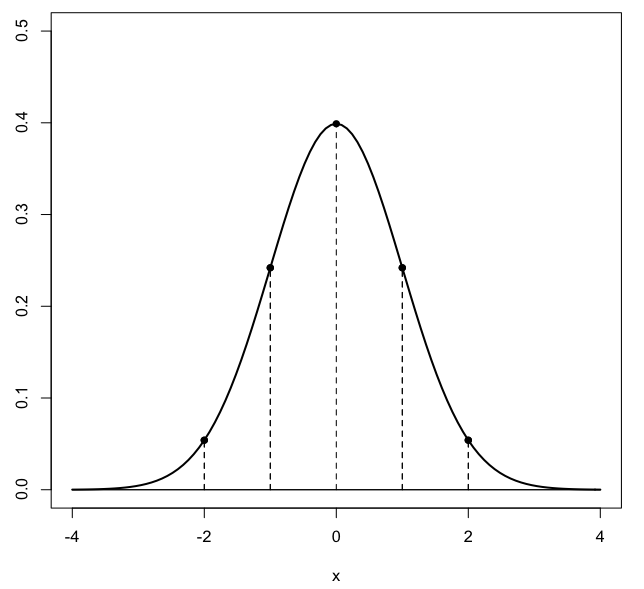
\includegraphics [scale=0.4] {gauss3.png} \end{center}

\title{Boundedness}
\date{}

\begin{document}
\maketitle
\Large

\section{f is bounded above}

A continuous function on a closed bounded interval is bounded.

\subsection*{theorem}

If $f$ is continuous on $[a,b]$ then $f$ is bounded above on $[a,b]$, that is, there is some number $M$ such that $f(x) \le M$ for all $x$ in $[a,b]$.

\begin{center} 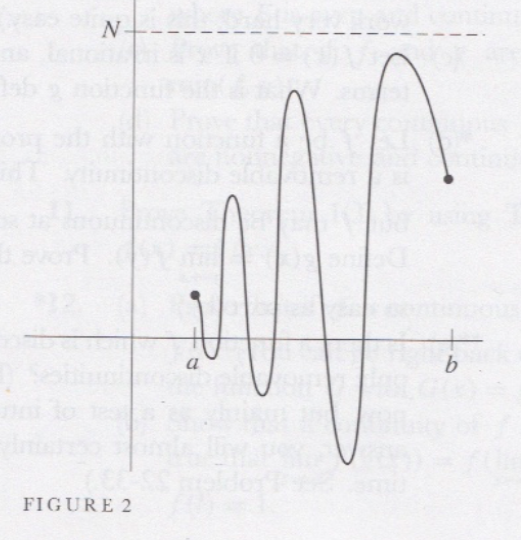
\includegraphics [scale=0.4] {spivak2.png} \end{center}

\url{www-history.mcs.st-and.ac.uk/~john/analysis/Lectures/L21.html}

\subsection*{restatement}

A continuous function on a closed bounded interval is bounded and achieves its bounds.

\section{Spivak}

\subsection*{preliminary theorem}

If $f$ is continuous at $a$, then there is a $\delta > 0$ such that $f$ is bounded above on the interval $[a - \delta, a + \delta]$.

\subsection*{proof}

By the definition of continuity, for every $\epsilon > 0$, there is a $\delta > 0$ such that if
\[ |x - a| < \delta \]
then
\[ |f(x) - f(a)| < \epsilon \]

Pick any $\epsilon$, for example $\epsilon = 1$.  Then we have that if $|x - a| < \delta$
\[  |f(x) - f(a)| < 1 \]
\[ - 1 < f(x) - f(a) < 1 \]
\[ f(a) - 1 < f(x) <  f(a) + 1 \]
On the interval $(a - \delta, a + \delta)$, $f(x)$ is bounded above by $f(a) + 1$.

$\square$

Define the set $A$ as all those values in the interval from $a$ to the "right" for which the function $f(x)$ is bounded above:

$A = \{ x: a \le x \le b$, and $f$ is bounded above on $[a,x]\}$

Clearly, $A \ne \varnothing$, since $a \in A$.

$A$ is bounded above (by $b$) so $A$ has a least upper bound, $\alpha$.

(Note:  the set $A$ is bounded above, but the theorem is about the function $f$, that is, it applies to $\{ f(y) : a \le y \le x \} $).

We claim that $\alpha = b$.

Note first that $\alpha$ cannot be equal to $a$, since $a$ is in $A$ and since there is a $\delta$ such that $f$ is bounded on $[x: a \le x \le a + \delta]$.

Suppose instead that $\alpha < b$ (it cannot be greater).

By the preliminary theorem, there exists a $\delta > 0$ such that $f$ is bounded on $[a, a + \delta]$.

Since $\alpha$ is the \emph{least} upper bound of $A$, there is some $x_0$ in $A$ satisfying $\alpha - \delta < x_0 < \alpha$.  This means that $f$ is bounded on $[a,x_0]$.

But if $x_1$ is any number with $\alpha < x_1 < \alpha + \delta$, then $f$ is also bounded on $[x_0,x_1]$.  Then $f$ is bounded on $[x_0,x_1]$.  Therefore, $f$ is bounded on $[a, x_1]$, so $x_1$ is in $A$, which contradicts the fact that $\alpha$ is an upper bound for $A$.

This contradiction shows that $\alpha = b$.

There is an additional small bit extending the interval to include $b$.

\section{other people}

\subsection*{proof}

Suppose $f$ is defined and continuous at every point of the interval $[a,b]$.

If $f$ were not bounded above, we could find a point $x_1$ in $[a,b]$ with $f(x_1) > 1$, a point $x_2$ with $f(x_2) > 2$, and so on.

Consider the sequence $(x_n)$.  By the Bolzano-Weierstrass Theorem, it has a subsequence $({x_i}_j)$ which converges.  

Call that point $\alpha \in [a,b]$.

By our construction, $f({x_i}_j)$ is unbounded.

But by the continuity of $f$, this sequence should converge to $f(\alpha)$, and we have a contradiction.

To show that $f$ attains its bounds, take $M$ to be the least upper bound of the set $X = \{ \ f(x) \ | \ x \in [a,b] \ \}$.  We need to find a point $\beta \in [a,b]$ with $f(\beta) = M$. 

To do this we construct a sequence in the following way:  for each $n \in \mathbb{N}$, let $x_n$ be a point for which $|M - f(x_n)| < 1/n$.

Such a point must exist because otherwise $M - 1/n$ would be an upper bound of $X$.  

Some subsequence of $(x_1, x_2 \dots)$ converges to $\beta$ (say) and 
\[ (f(x_1), f(x_2), \dots) \rightarrow M \]
and so by continuity $f(\beta) = M$, as required.

\subsection*{proof 2}
Let $\mathbf{A} = [a,b]$.

Clearly, $\mathbf{A} \ne \varnothing$ ($\mathbf{A}$ is not empty), since $a$ is in $\mathbf{A}$, and $\mathbf{A}$ is bounded above by $b$.  So, $\mathbf{A}$ has a least upper bound, $\alpha$.

Assume that $f$ is \emph{not} bounded above.

What does that mean?  It means that no matter what $n \in \mathbb{N}$ we choose, we can find $x_n \in \mathbf{A}: f(x_n) > n$.

Since $\mathbf{A}$ is bounded, and the $x_n$ are in $\mathbf{A}$, the sequence $(x_n)$ is bounded.  By the Bolzano-Weierstrass theorem, $(x_n)$ has a convergent subsequence $(x_nk)$.  So it has a limit, $L$.

Since all the terms of $(x_nk)$ are in $\mathbf{A}$, so is $L$.

But $f((x_nk))$ is unbounded.

By the Sequential Criterion for Continuity (an “if and only if” theorem), we conclude that lim $f((x_nk)) = f(L)$.

This is a contradiction.  Therefore, $f$ is bounded above.

\end{document}}